\documentclass{beamer}

\usepackage[utf8]{inputenc}

\usepackage{relsize}
\usepackage{graphicx}
\usepackage{subcaption}
\usepackage{etoolbox}
\usepackage{amssymb}
\usepackage{siunitx}
\usepackage{verbatim} 
\usepackage{wrapfig}
\usepackage{float}
\usepackage{boldline} 

\usepackage{colortbl}
\usepackage{xcolor}

\usepackage{tabularx}


\newcommand{\todo}[1]{\textcolor{red}{TODO: #1}\PackageWarning{TODO:}{#1!}}


\newcommand{\gc}{\cellcolor[HTML]{cccccc}}


\usetheme{Madrid}

%Information to be included in the title page:
\title{PQC Status Vienna}
\author{Maximilian Babeluk}
\institute{}
\date{April 20$^{th}$ 2021}

\graphicspath{{plots/}{imgs/}}

\makeatletter
\newcommand\appendtographicspath[1]{%
	\g@addto@macro\Ginput@path{#1}%
}
\makeatother



\usepackage{tikz}
\usetikzlibrary{fadings,shapes.arrows,shadows}
\usepackage{varwidth}

\usepackage{xparse}



\usepackage{graphicx}
\usetikzlibrary{calc}

\definecolor{dgreen}{RGB}{0, 124, 0}
\definecolor{dorange}{RGB}{200, 150, 0}

\newcommand\myheading[1]{%
	\par\bigskip
	{\Large\bfseries#1}\par\smallskip}


\newcolumntype{L}[1]{>{\raggedright\arraybackslash}p{#1}}

\begin{document}
	
	\frame{\titlepage}
	
	\setbeamertemplate{frametitle}[default][center]
	
	\addtobeamertemplate{frametitle}{}{%
		\begin{tikzpicture}[remember picture,overlay]
		\node[anchor=north east,yshift=4pt] at (current page.north east) {
\includegraphics[height=0.9cm]{imgs/oeaw.jpg}};
		
		\node[anchor=north west,yshift=4pt] at (current page.north west) {
\includegraphics[height=0.9cm]{imgs/cms.png}};
		\node[anchor=north west,yshift=4pt, xshift=1cm] at (current page.north west) {
\includegraphics[height=0.9cm]{imgs/hephyalt.png}};
		
	\end{tikzpicture}}

	
	
	
	\begin{frame}
		\frametitle{PQC Status}
		
		\begin{itemize}
			\item{New contacting procedure:}
			\begin{itemize}
				\item{Align XY position with camera}
				\item{Use LCR-meter for touchdown}
				\item{Rp in Cp/Rp equivalent circuit as contact-quality measure}
				\item{Across all needles (all VdP on flute1 parallel)}
			\end{itemize}
			\item{Automatic re-measurement for suspicious results}

		\end{itemize}
	
	
		\begin{center}
			\fontsize{7pt}{9pt}\selectfont
			\begin{tabular}{ |l|l|l|l|L{2.5cm}|l|L{1.5cm}| }
				\hline
				 Batch & Type & Wafers & Tested & Status & Date & Link \\
				 \hline
				 VPX35953 & 2-S & 40 pcs & 6+3 & \ \color{dgreen} OK \color{dorange} (BD pending, p-stop inhom.) & April 13$^{th}$ 2021 & \fontsize{5pt}{6pt}\selectfont \href{https://indico.cern.ch/event/1028589/}{https://indico.cern.ch/event/1028589/} \\
\hline
				VPX35496 & PS-P & 44 pcs & 8+0 & \ \color{dgreen} OK \color{dorange} (low Bulk resistivity) & today & \fontsize{5pt}{6pt}\selectfont \href{https://indico.cern.ch/event/1028816/}{https://indico.cern.ch/event/1028816/} \\
\hline
				VPX35499 & PS-P & 47 pcs & & pending & & \\
				 \hline
			\end{tabular}
		\end{center}
	
	\end{frame}
	
	
	\def\batch{VPX35496}
	
	\begin{frame}
		\frametitle{\batch: Flute 1}
		





    



\def\nanval{\cellcolor[HTML]{aa0000}}
\def\highval{\cellcolor[HTML]{ff9900}}
\def\lowval{\cellcolor[HTML]{ffff00}}
\def\okval{\cellcolor[HTML]{ffffff}}
\def\notmeasval{\cellcolor[HTML]{d4fcfc}}

\newcolumntype{L}[1]{>{\raggedright\arraybackslash}p{#1}}
\newcolumntype{C}[1]{>{\centering\arraybackslash}p{#1}}
\newcolumntype{R}[1]{>{\raggedleft\arraybackslash}p{#1}}

\begin{center}
    \fontsize{4pt}{5pt}\selectfont
    \setlength{\tabcolsep}{0.35em} % for the horizontal padding
    \begin{tabular}{ |l|R{0.6cm}|R{0.6cm}|R{0.6cm}|R{0.6cm}|R{0.6cm}|R{0.6cm}|R{0.6cm}|R{0.6cm}|R{0.6cm}|R{0.6cm}|R{0.6cm}|R{0.6cm}|R{0.6cm}| }
        \hline
         & FET & \multicolumn{4}{ c|}{MOS Quarter} & \multicolumn{2}{ c|}{Polysilicon VdP} & \multicolumn{2}{ c|}{n+ VdP} & \multicolumn{2}{ c|}{p-stop VdP} & \multicolumn{2}{ c|}{Capacitor} \\
        \hline
        \detokenize{  } & \detokenize{ fet } & \detokenize{ v_fb } & \detokenize{ c_acc } & \detokenize{ t_ox } & \detokenize{ n_ox } & \detokenize{ vdpPoly } & \detokenize{ vdpPoly_r } & \detokenize{ vdpN } & \detokenize{ vdpN_r } & \detokenize{ vdpPstp } & \detokenize{ vdpPstp_r } & \detokenize{ cap_l } & \detokenize{ cap_r } \\

        \hline
        \detokenize{  } & \detokenize{ V } & \detokenize{ V } & \detokenize{ pF } & \detokenize{ nm } & \detokenize{ 1E10cm^-3 } & \detokenize{ kOhm/sq } & \detokenize{ kOhm/sq } & \detokenize{ Ohm/sq } & \detokenize{ Ohm/sq } & \detokenize{ kOhm/sq } & \detokenize{ kOhm/sq } & \detokenize{ pF } & \detokenize{ pF } \\

        \hline
        
        \detokenize{ HPK_VPX35496_001_PSP_HM_EL } & \lowval 2.23 & \highval 5.21 & \okval 87.9 & \okval 653.3 & \highval 19.5 & \notmeasval --- & \notmeasval --- & \okval 35.3 & \okval 35.1 & \okval 18.6 & \okval 18.6 & \okval 3.46 & \okval 3.31 \\
\detokenize{ HPK_VPX35496_001_PSP_HM_ER } & \lowval 2.57 & \highval 4.72 & \okval 86.6 & \okval 662.9 & \highval 17.6 & \notmeasval --- & \notmeasval --- & \okval 35.1 & \okval 35.3 & \okval 18.5 & \okval 18.5 & \okval 3.36 & \okval 3.22 \\
\detokenize{ HPK_VPX35496_001_PSP_HM_WL } & \lowval 2.59 & \highval 4.71 & \okval 86.7 & \okval 662.2 & \highval 17.6 & \notmeasval --- & \notmeasval --- & \okval 35.5 & \okval 35.3 & \okval 18.5 & \okval 18.5 & \okval 3.39 & \okval 3.24 \\
\detokenize{ HPK_VPX35496_001_PSP_HM_WR } & \lowval 2.19 & \highval 5.38 & \okval 87.4 & \okval 657.1 & \highval 19.9 & \notmeasval --- & \notmeasval --- & \okval 35.3 & \okval 35.4 & \okval 18.7 & \okval 18.7 & \okval 3.43 & \okval 3.29 \\
\detokenize{ HPK_VPX35496_002_PSP_HM_EL } & \nanval failed & \highval 5.28 & \okval 87.7 & \okval 654.6 & \highval 19.7 & \notmeasval --- & \notmeasval --- & \nanval failed & \nanval failed & \nanval failed & \nanval failed & \okval 3.39 & \okval 3.27 \\
\detokenize{ HPK_VPX35496_002_PSP_HM_ER } & \lowval 2.50 & \highval 4.80 & \okval 86.9 & \okval 660.6 & \highval 17.9 & \notmeasval --- & \notmeasval --- & \okval 35.2 & \okval 35.3 & \okval 18.6 & \okval 18.6 & \okval 3.33 & \okval 3.21 \\
\detokenize{ HPK_VPX35496_002_PSP_HM_WL } & \lowval 2.64 & \highval 4.63 & \okval 86.7 & \okval 662.1 & \highval 17.3 & \notmeasval --- & \notmeasval --- & \okval 35.6 & \okval 35.3 & \okval 18.5 & \okval 18.5 & \okval 3.37 & \okval 3.25 \\
\detokenize{ HPK_VPX35496_002_PSP_HM_WR } & \lowval 2.23 & \highval 5.28 & \okval 87.7 & \okval 655.0 & \highval 19.6 & \notmeasval --- & \notmeasval --- & \okval 35.3 & \okval 35.4 & \okval 18.7 & \okval 18.7 & \okval 3.42 & \okval 3.29 \\
\detokenize{ HPK_VPX35496_010_PSP_HM_EL } & \lowval 2.25 & \highval 5.20 & \okval 88.1 & \okval 651.7 & \highval 19.5 & \notmeasval --- & \notmeasval --- & \okval 35.4 & \okval 35.3 & \okval 18.6 & \okval 18.6 & \okval 3.48 & \okval 3.34 \\
\detokenize{ HPK_VPX35496_010_PSP_HM_ER } & \lowval 2.47 & \highval 4.88 & \okval 87.0 & \okval 660.6 & \highval 18.2 & \notmeasval --- & \notmeasval --- & \okval 35.3 & \okval 35.3 & \okval 18.7 & \okval 18.7 & \okval 3.38 & \okval 3.25 \\
\detokenize{ HPK_VPX35496_010_PSP_HM_WL } & \lowval 2.60 & \highval 4.73 & \okval 86.7 & \okval 662.8 & \highval 17.6 & \notmeasval --- & \notmeasval --- & \okval 35.7 & \okval 35.4 & \okval 18.6 & \okval 18.6 & \okval 3.36 & \okval 3.22 \\
\detokenize{ HPK_VPX35496_010_PSP_HM_WR } & \lowval 2.26 & \highval 5.30 & \okval 87.0 & \okval 660.1 & \highval 19.5 & \notmeasval --- & \notmeasval --- & \okval 35.4 & \okval 35.4 & \okval 18.7 & \okval 18.7 & \okval 3.41 & \okval 3.27 \\
\detokenize{ HPK_VPX35496_017_PSP_HM_EL } & \lowval 2.28 & \highval 5.12 & \okval 87.8 & \okval 654.0 & \highval 19.2 & \notmeasval --- & \notmeasval --- & \okval 35.2 & \okval 35.3 & \okval 18.6 & \okval 18.6 & \okval 3.38 & \okval 3.26 \\
\detokenize{ HPK_VPX35496_017_PSP_HM_ER } & \lowval 2.49 & \highval 4.86 & \okval 87.1 & \okval 659.1 & \highval 18.1 & \notmeasval --- & \notmeasval --- & \okval 35.2 & \okval 35.4 & \okval 18.7 & \okval 18.6 & \okval 3.32 & \okval 3.21 \\
\detokenize{ HPK_VPX35496_017_PSP_HM_WL } & \lowval 2.41 & \highval 4.79 & \okval 86.6 & \okval 662.9 & \highval 17.8 & \notmeasval --- & \notmeasval --- & \okval 35.7 & \okval 35.4 & \okval 18.6 & \okval 18.7 & \okval 3.35 & \okval 3.23 \\
\detokenize{ HPK_VPX35496_017_PSP_HM_WR } & \lowval 2.26 & \highval 5.25 & \okval 87.6 & \okval 655.9 & \highval 19.5 & \notmeasval --- & \notmeasval --- & \okval 35.4 & \okval 35.4 & \okval 18.8 & \okval 18.7 & \okval 3.40 & \okval 3.28 \\
\detokenize{ HPK_VPX35496_026_PSP_HM_EL } & \lowval 2.38 & \highval 5.00 & \okval 88.2 & \okval 651.4 & \highval 18.8 & \notmeasval --- & \notmeasval --- & \okval 35.3 & \okval 35.1 & \okval 18.4 & \okval 18.5 & \okval 3.45 & \okval 3.30 \\
\detokenize{ HPK_VPX35496_026_PSP_HM_ER } & \lowval 2.70 & \highval 4.37 & \okval 87.4 & \okval 657.1 & \highval 16.6 & \notmeasval --- & \notmeasval --- & \okval 35.0 & \okval 35.3 & \okval 18.5 & \okval 18.5 & \okval 3.37 & \okval 3.23 \\
\detokenize{ HPK_VPX35496_026_PSP_HM_WL } & \lowval 2.78 & \highval 4.30 & \okval 87.1 & \okval 659.3 & \highval 16.3 & \notmeasval --- & \notmeasval --- & \okval 35.4 & \okval 35.2 & \okval 18.5 & \okval 18.5 & \okval 3.38 & \okval 3.24 \\
\detokenize{ HPK_VPX35496_026_PSP_HM_WR } & \lowval 2.35 & \highval 5.11 & \okval 87.6 & \okval 655.4 & \highval 19.1 & \notmeasval --- & \notmeasval --- & \okval 35.3 & \okval 35.5 & \okval 18.5 & \okval 18.5 & \okval 3.42 & \okval 3.28 \\
\detokenize{ HPK_VPX35496_032_PSP_HM_EL } & \lowval 2.38 & \highval 4.99 & \okval 88.0 & \okval 652.7 & \highval 18.7 & \notmeasval --- & \notmeasval --- & \okval 35.2 & \okval 35.2 & \okval 18.6 & \okval 18.7 & \okval 3.36 & \okval 3.24 \\
\detokenize{ HPK_VPX35496_032_PSP_HM_ER } & \lowval 2.70 & \highval 4.34 & \okval 87.7 & \okval 655.0 & \highval 16.5 & \notmeasval --- & \notmeasval --- & \okval 35.1 & \okval 35.2 & \okval 18.6 & \okval 18.6 & \okval 3.33 & \okval 3.21 \\
\detokenize{ HPK_VPX35496_032_PSP_HM_WL } & \lowval 2.75 & \highval 4.25 & \okval 88.0 & \okval 652.5 & \highval 16.3 & \notmeasval --- & \notmeasval --- & \okval 35.6 & \okval 35.2 & \okval 18.6 & \okval 18.6 & \okval 3.39 & \okval 3.26 \\
\detokenize{ HPK_VPX35496_032_PSP_HM_WR } & \lowval 2.37 & \highval 5.02 & \okval 88.0 & \okval 652.7 & \highval 18.9 & \notmeasval --- & \notmeasval --- & \okval 35.3 & \okval 35.3 & \okval 18.7 & \okval 18.7 & \okval 3.41 & \okval 3.28 \\
\detokenize{ HPK_VPX35496_040_PSP_HM_EL } & \lowval 2.31 & \highval 5.00 & \okval 88.4 & \okval 649.5 & \highval 18.9 & \notmeasval --- & \notmeasval --- & \okval 35.3 & \okval 35.2 & \okval 18.7 & \okval 18.8 & \okval 3.24 & \okval 3.11 \\
\detokenize{ HPK_VPX35496_040_PSP_HM_ER } & \lowval 2.63 & \highval 4.47 & \okval 88.0 & \okval 653.0 & \highval 17.0 & \notmeasval --- & \notmeasval --- & \okval 35.1 & \okval 35.4 & \okval 18.7 & \okval 18.7 & \okval 3.16 & \okval 3.04 \\
\detokenize{ HPK_VPX35496_040_PSP_HM_WL } & \lowval 2.68 & \highval 4.33 & \okval 88.1 & \okval 652.0 & \highval 16.6 & \notmeasval --- & \notmeasval --- & \okval 35.6 & \okval 35.2 & \okval 18.7 & \okval 18.7 & \okval 3.18 & \okval 3.06 \\
\detokenize{ HPK_VPX35496_040_PSP_HM_WR } & \lowval 2.26 & \highval 5.09 & \okval 88.3 & \okval 650.8 & \highval 19.1 & \notmeasval --- & \notmeasval --- & \okval 35.4 & \okval 35.4 & \okval 18.8 & \okval 18.8 & \okval 3.22 & \okval 3.10 \\
\detokenize{ HPK_VPX35496_044_PSP_HM_EL } & \lowval 2.27 & \highval 5.12 & \okval 87.8 & \okval 654.3 & \highval 19.1 & \notmeasval --- & \notmeasval --- & \okval 35.1 & \okval 35.2 & \okval 18.9 & \okval 18.8 & \okval 3.14 & \okval 3.03 \\
\detokenize{ HPK_VPX35496_044_PSP_HM_ER } & \lowval 2.53 & \highval 4.60 & \okval 87.9 & \okval 653.4 & \highval 17.4 & \notmeasval --- & \notmeasval --- & \okval 35.1 & \okval 35.3 & \okval 18.9 & \okval 18.9 & \okval 3.12 & \okval 3.02 \\
\detokenize{ HPK_VPX35496_044_PSP_HM_WL } & \lowval 2.63 & \highval 4.47 & \okval 88.5 & \okval 648.9 & \highval 17.1 & \notmeasval --- & \notmeasval --- & \okval 35.7 & \okval 35.4 & \okval 18.9 & \okval 18.9 & \okval 3.19 & \okval 3.09 \\
\detokenize{ HPK_VPX35496_044_PSP_HM_WR } & \lowval 2.20 & \highval 5.16 & \okval 88.8 & \okval 646.8 & \highval 19.5 & \notmeasval --- & \notmeasval --- & \okval 35.5 & \okval 35.5 & \okval 18.9 & \okval 18.9 & \okval 3.23 & \okval 3.12 \\
        \hline
        \detokenize{ Median } & \okval  nan & \okval  nan & \okval 87.7 & \okval 654.8 & \okval  nan & \okval 0.00 & \okval 0.00 & \okval 35.3 & \okval 35.3 & \okval 18.6 & \okval 18.7 & \okval 3.37 & \okval 3.24 \\
\detokenize{ Average } & \okval  nan & \okval  nan & \okval 87.6 & \okval 655.6 & \okval  nan & \okval 0.00 & \okval 0.00 & \okval 35.4 & \okval 35.3 & \okval 18.7 & \okval 18.7 & \okval 3.34 & \okval 3.21 \\
\detokenize{ Std dev. } & \okval  nan & \okval  nan & \okval  0.6 & \okval  4.4 & \okval  nan & \okval 0.00 & \okval 0.00 & \okval  0.2 & \okval  0.1 & \okval  0.1 & \okval  0.1 & \okval 0.10 & \okval 0.09 \\
\detokenize{ OK/Tot. } & \okval 0/32 & \okval 0/32 & \okval 32/32 & \okval 32/32 & \okval 0/32 & \okval 1/1 & \okval 1/1 & \okval 31/32 & \okval 31/32 & \okval 31/32 & \okval 31/32 & \okval 32/32 & \okval 32/32 \\
\detokenize{ OK (rel) } & \okval 0.00 & \okval 0.00 & \okval 1.00 & \okval 1.00 & \okval 0.00 & \okval 1.00 & \okval 1.00 & \okval 0.97 & \okval 0.97 & \okval 0.97 & \okval 0.97 & \okval 1.00 & \okval 1.00 \\

        \hline
    \end{tabular}
\end{center}

	\end{frame}


	\begin{frame}
		\frametitle{\batch: Flute 1}
		





    



\def\nanval{\cellcolor[HTML]{aa0000}}
\def\highval{\cellcolor[HTML]{ff9900}}
\def\lowval{\cellcolor[HTML]{ffff00}}
\def\okval{\cellcolor[HTML]{ffffff}}
\def\notmeasval{\cellcolor[HTML]{d4fcfc}}

\newcolumntype{L}[1]{>{\raggedright\arraybackslash}p{#1}}
\newcolumntype{C}[1]{>{\centering\arraybackslash}p{#1}}
\newcolumntype{R}[1]{>{\raggedleft\arraybackslash}p{#1}}

\begin{center}
    \fontsize{4pt}{5pt}\selectfont
    \setlength{\tabcolsep}{0.35em} % for the horizontal padding
    \begin{tabular}{ |l|R{0.6cm}|R{0.6cm}|R{0.6cm}|R{0.6cm}|R{0.6cm}|R{0.6cm}|R{0.6cm}|R{0.6cm}|R{0.6cm}|R{0.6cm}|R{0.6cm}|R{0.6cm}|R{0.6cm}| }
        \hline
         & FET & \multicolumn{4}{ c|}{MOS Quarter} & \multicolumn{2}{ c|}{Polysilicon VdP} & \multicolumn{2}{ c|}{n+ VdP} & \multicolumn{2}{ c|}{p-stop VdP} & \multicolumn{2}{ c|}{Capacitor} \\
        \hline
        \detokenize{  } & \detokenize{ fet } & \detokenize{ v_fb } & \detokenize{ c_acc } & \detokenize{ t_ox } & \detokenize{ n_ox } & \detokenize{ vdpPoly } & \detokenize{ vdpPoly_r } & \detokenize{ vdpN } & \detokenize{ vdpN_r } & \detokenize{ vdpPstp } & \detokenize{ vdpPstp_r } & \detokenize{ cap_l } & \detokenize{ cap_r } \\

        \hline
        \detokenize{  } & \detokenize{ V } & \detokenize{ V } & \detokenize{ pF } & \detokenize{ nm } & \detokenize{ 1E10cm^-3 } & \detokenize{ kOhm/sq } & \detokenize{ kOhm/sq } & \detokenize{ Ohm/sq } & \detokenize{ Ohm/sq } & \detokenize{ kOhm/sq } & \detokenize{ kOhm/sq } & \detokenize{ pF } & \detokenize{ pF } \\

        \hline
        
        \detokenize{ HPK_VPX35496_001_PSP_HM_EL } & \lowval 2.23 & \highval 5.21 & \okval 87.9 & \okval 653.3 & \highval 19.5 & \notmeasval --- & \notmeasval --- & \okval 35.3 & \okval 35.1 & \okval 18.6 & \okval 18.6 & \okval 3.46 & \okval 3.31 \\
\detokenize{ HPK_VPX35496_001_PSP_HM_ER } & \lowval 2.57 & \highval 4.72 & \okval 86.6 & \okval 662.9 & \highval 17.6 & \notmeasval --- & \notmeasval --- & \okval 35.1 & \okval 35.3 & \okval 18.5 & \okval 18.5 & \okval 3.36 & \okval 3.22 \\
\detokenize{ HPK_VPX35496_001_PSP_HM_WL } & \lowval 2.59 & \highval 4.71 & \okval 86.7 & \okval 662.2 & \highval 17.6 & \notmeasval --- & \notmeasval --- & \okval 35.5 & \okval 35.3 & \okval 18.5 & \okval 18.5 & \okval 3.39 & \okval 3.24 \\
\detokenize{ HPK_VPX35496_001_PSP_HM_WR } & \lowval 2.19 & \highval 5.38 & \okval 87.4 & \okval 657.1 & \highval 19.9 & \notmeasval --- & \notmeasval --- & \okval 35.3 & \okval 35.4 & \okval 18.7 & \okval 18.7 & \okval 3.43 & \okval 3.29 \\
\detokenize{ HPK_VPX35496_002_PSP_HM_EL } & \nanval failed & \highval 5.28 & \okval 87.7 & \okval 654.6 & \highval 19.7 & \notmeasval --- & \notmeasval --- & \nanval failed & \nanval failed & \nanval failed & \nanval failed & \okval 3.39 & \okval 3.27 \\
\detokenize{ HPK_VPX35496_002_PSP_HM_ER } & \lowval 2.50 & \highval 4.80 & \okval 86.9 & \okval 660.6 & \highval 17.9 & \notmeasval --- & \notmeasval --- & \okval 35.2 & \okval 35.3 & \okval 18.6 & \okval 18.6 & \okval 3.33 & \okval 3.21 \\
\detokenize{ HPK_VPX35496_002_PSP_HM_WL } & \lowval 2.64 & \highval 4.63 & \okval 86.7 & \okval 662.1 & \highval 17.3 & \notmeasval --- & \notmeasval --- & \okval 35.6 & \okval 35.3 & \okval 18.5 & \okval 18.5 & \okval 3.37 & \okval 3.25 \\
\detokenize{ HPK_VPX35496_002_PSP_HM_WR } & \lowval 2.23 & \highval 5.28 & \okval 87.7 & \okval 655.0 & \highval 19.6 & \notmeasval --- & \notmeasval --- & \okval 35.3 & \okval 35.4 & \okval 18.7 & \okval 18.7 & \okval 3.42 & \okval 3.29 \\
\detokenize{ HPK_VPX35496_010_PSP_HM_EL } & \lowval 2.25 & \highval 5.20 & \okval 88.1 & \okval 651.7 & \highval 19.5 & \notmeasval --- & \notmeasval --- & \okval 35.4 & \okval 35.3 & \okval 18.6 & \okval 18.6 & \okval 3.48 & \okval 3.34 \\
\detokenize{ HPK_VPX35496_010_PSP_HM_ER } & \lowval 2.47 & \highval 4.88 & \okval 87.0 & \okval 660.6 & \highval 18.2 & \notmeasval --- & \notmeasval --- & \okval 35.3 & \okval 35.3 & \okval 18.7 & \okval 18.7 & \okval 3.38 & \okval 3.25 \\
\detokenize{ HPK_VPX35496_010_PSP_HM_WL } & \lowval 2.60 & \highval 4.73 & \okval 86.7 & \okval 662.8 & \highval 17.6 & \notmeasval --- & \notmeasval --- & \okval 35.7 & \okval 35.4 & \okval 18.6 & \okval 18.6 & \okval 3.36 & \okval 3.22 \\
\detokenize{ HPK_VPX35496_010_PSP_HM_WR } & \lowval 2.26 & \highval 5.30 & \okval 87.0 & \okval 660.1 & \highval 19.5 & \notmeasval --- & \notmeasval --- & \okval 35.4 & \okval 35.4 & \okval 18.7 & \okval 18.7 & \okval 3.41 & \okval 3.27 \\
\detokenize{ HPK_VPX35496_017_PSP_HM_EL } & \lowval 2.28 & \highval 5.12 & \okval 87.8 & \okval 654.0 & \highval 19.2 & \notmeasval --- & \notmeasval --- & \okval 35.2 & \okval 35.3 & \okval 18.6 & \okval 18.6 & \okval 3.38 & \okval 3.26 \\
\detokenize{ HPK_VPX35496_017_PSP_HM_ER } & \lowval 2.49 & \highval 4.86 & \okval 87.1 & \okval 659.1 & \highval 18.1 & \notmeasval --- & \notmeasval --- & \okval 35.2 & \okval 35.4 & \okval 18.7 & \okval 18.6 & \okval 3.32 & \okval 3.21 \\
\detokenize{ HPK_VPX35496_017_PSP_HM_WL } & \lowval 2.41 & \highval 4.79 & \okval 86.6 & \okval 662.9 & \highval 17.8 & \notmeasval --- & \notmeasval --- & \okval 35.7 & \okval 35.4 & \okval 18.6 & \okval 18.7 & \okval 3.35 & \okval 3.23 \\
\detokenize{ HPK_VPX35496_017_PSP_HM_WR } & \lowval 2.26 & \highval 5.25 & \okval 87.6 & \okval 655.9 & \highval 19.5 & \notmeasval --- & \notmeasval --- & \okval 35.4 & \okval 35.4 & \okval 18.8 & \okval 18.7 & \okval 3.40 & \okval 3.28 \\
\detokenize{ HPK_VPX35496_026_PSP_HM_EL } & \lowval 2.38 & \highval 5.00 & \okval 88.2 & \okval 651.4 & \highval 18.8 & \notmeasval --- & \notmeasval --- & \okval 35.3 & \okval 35.1 & \okval 18.4 & \okval 18.5 & \okval 3.45 & \okval 3.30 \\
\detokenize{ HPK_VPX35496_026_PSP_HM_ER } & \lowval 2.70 & \highval 4.37 & \okval 87.4 & \okval 657.1 & \highval 16.6 & \notmeasval --- & \notmeasval --- & \okval 35.0 & \okval 35.3 & \okval 18.5 & \okval 18.5 & \okval 3.37 & \okval 3.23 \\
\detokenize{ HPK_VPX35496_026_PSP_HM_WL } & \lowval 2.78 & \highval 4.30 & \okval 87.1 & \okval 659.3 & \highval 16.3 & \notmeasval --- & \notmeasval --- & \okval 35.4 & \okval 35.2 & \okval 18.5 & \okval 18.5 & \okval 3.38 & \okval 3.24 \\
\detokenize{ HPK_VPX35496_026_PSP_HM_WR } & \lowval 2.35 & \highval 5.11 & \okval 87.6 & \okval 655.4 & \highval 19.1 & \notmeasval --- & \notmeasval --- & \okval 35.3 & \okval 35.5 & \okval 18.5 & \okval 18.5 & \okval 3.42 & \okval 3.28 \\
\detokenize{ HPK_VPX35496_032_PSP_HM_EL } & \lowval 2.38 & \highval 4.99 & \okval 88.0 & \okval 652.7 & \highval 18.7 & \notmeasval --- & \notmeasval --- & \okval 35.2 & \okval 35.2 & \okval 18.6 & \okval 18.7 & \okval 3.36 & \okval 3.24 \\
\detokenize{ HPK_VPX35496_032_PSP_HM_ER } & \lowval 2.70 & \highval 4.34 & \okval 87.7 & \okval 655.0 & \highval 16.5 & \notmeasval --- & \notmeasval --- & \okval 35.1 & \okval 35.2 & \okval 18.6 & \okval 18.6 & \okval 3.33 & \okval 3.21 \\
\detokenize{ HPK_VPX35496_032_PSP_HM_WL } & \lowval 2.75 & \highval 4.25 & \okval 88.0 & \okval 652.5 & \highval 16.3 & \notmeasval --- & \notmeasval --- & \okval 35.6 & \okval 35.2 & \okval 18.6 & \okval 18.6 & \okval 3.39 & \okval 3.26 \\
\detokenize{ HPK_VPX35496_032_PSP_HM_WR } & \lowval 2.37 & \highval 5.02 & \okval 88.0 & \okval 652.7 & \highval 18.9 & \notmeasval --- & \notmeasval --- & \okval 35.3 & \okval 35.3 & \okval 18.7 & \okval 18.7 & \okval 3.41 & \okval 3.28 \\
\detokenize{ HPK_VPX35496_040_PSP_HM_EL } & \lowval 2.31 & \highval 5.00 & \okval 88.4 & \okval 649.5 & \highval 18.9 & \notmeasval --- & \notmeasval --- & \okval 35.3 & \okval 35.2 & \okval 18.7 & \okval 18.8 & \okval 3.24 & \okval 3.11 \\
\detokenize{ HPK_VPX35496_040_PSP_HM_ER } & \lowval 2.63 & \highval 4.47 & \okval 88.0 & \okval 653.0 & \highval 17.0 & \notmeasval --- & \notmeasval --- & \okval 35.1 & \okval 35.4 & \okval 18.7 & \okval 18.7 & \okval 3.16 & \okval 3.04 \\
\detokenize{ HPK_VPX35496_040_PSP_HM_WL } & \lowval 2.68 & \highval 4.33 & \okval 88.1 & \okval 652.0 & \highval 16.6 & \notmeasval --- & \notmeasval --- & \okval 35.6 & \okval 35.2 & \okval 18.7 & \okval 18.7 & \okval 3.18 & \okval 3.06 \\
\detokenize{ HPK_VPX35496_040_PSP_HM_WR } & \lowval 2.26 & \highval 5.09 & \okval 88.3 & \okval 650.8 & \highval 19.1 & \notmeasval --- & \notmeasval --- & \okval 35.4 & \okval 35.4 & \okval 18.8 & \okval 18.8 & \okval 3.22 & \okval 3.10 \\
\detokenize{ HPK_VPX35496_044_PSP_HM_EL } & \lowval 2.27 & \highval 5.12 & \okval 87.8 & \okval 654.3 & \highval 19.1 & \notmeasval --- & \notmeasval --- & \okval 35.1 & \okval 35.2 & \okval 18.9 & \okval 18.8 & \okval 3.14 & \okval 3.03 \\
\detokenize{ HPK_VPX35496_044_PSP_HM_ER } & \lowval 2.53 & \highval 4.60 & \okval 87.9 & \okval 653.4 & \highval 17.4 & \notmeasval --- & \notmeasval --- & \okval 35.1 & \okval 35.3 & \okval 18.9 & \okval 18.9 & \okval 3.12 & \okval 3.02 \\
\detokenize{ HPK_VPX35496_044_PSP_HM_WL } & \lowval 2.63 & \highval 4.47 & \okval 88.5 & \okval 648.9 & \highval 17.1 & \notmeasval --- & \notmeasval --- & \okval 35.7 & \okval 35.4 & \okval 18.9 & \okval 18.9 & \okval 3.19 & \okval 3.09 \\
\detokenize{ HPK_VPX35496_044_PSP_HM_WR } & \lowval 2.20 & \highval 5.16 & \okval 88.8 & \okval 646.8 & \highval 19.5 & \notmeasval --- & \notmeasval --- & \okval 35.5 & \okval 35.5 & \okval 18.9 & \okval 18.9 & \okval 3.23 & \okval 3.12 \\
        \hline
        \detokenize{ Median } & \okval  nan & \okval  nan & \okval 87.7 & \okval 654.8 & \okval  nan & \okval 0.00 & \okval 0.00 & \okval 35.3 & \okval 35.3 & \okval 18.6 & \okval 18.7 & \okval 3.37 & \okval 3.24 \\
\detokenize{ Average } & \okval  nan & \okval  nan & \okval 87.6 & \okval 655.6 & \okval  nan & \okval 0.00 & \okval 0.00 & \okval 35.4 & \okval 35.3 & \okval 18.7 & \okval 18.7 & \okval 3.34 & \okval 3.21 \\
\detokenize{ Std dev. } & \okval  nan & \okval  nan & \okval  0.6 & \okval  4.4 & \okval  nan & \okval 0.00 & \okval 0.00 & \okval  0.2 & \okval  0.1 & \okval  0.1 & \okval  0.1 & \okval 0.10 & \okval 0.09 \\
\detokenize{ OK/Tot. } & \okval 0/32 & \okval 0/32 & \okval 32/32 & \okval 32/32 & \okval 0/32 & \okval 1/1 & \okval 1/1 & \okval 31/32 & \okval 31/32 & \okval 31/32 & \okval 31/32 & \okval 32/32 & \okval 32/32 \\
\detokenize{ OK (rel) } & \okval 0.00 & \okval 0.00 & \okval 1.00 & \okval 1.00 & \okval 0.00 & \okval 1.00 & \okval 1.00 & \okval 0.97 & \okval 0.97 & \okval 0.97 & \okval 0.97 & \okval 1.00 & \okval 1.00 \\

        \hline
    \end{tabular}
\end{center}


		\begin{tikzpicture}[remember picture,overlay]
		
			\draw[draw=gray, fill=white, anchor=south west,inner sep=0pt] ($(current page.south west)+(0.8cm,3cm)$) rectangle ++(6.5cm,2.75cm);
			
			\node[anchor=south west,inner sep=0pt] at ($(current page.south west)+(0.8cm,3.25cm)$) {
				{\begin{varwidth}{\linewidth}		\begin{itemize}
					\fontsize{8pt}{10pt}\selectfont
					\item{Flatband voltage higher than 2-S/PS-S}
					\item{FET $V_{th}$ lower than in 2-S/PS-S}
					\item{Very good p-stop and FET $V_{th}$ homogenity}
					\item{No polysilicon layer on PS-P}
					\item{High capacitance on capacitor structure}
					\end{itemize}\end{varwidth}}
			};
		
		\end{tikzpicture}
	\end{frame}

	\begin{frame}
		\frametitle{\batch: Flute 2}
		






    



\def\nanval{\cellcolor[HTML]{aa0000}}
\def\highval{\cellcolor[HTML]{ff9900}}
\def\lowval{\cellcolor[HTML]{ffff00}}
\def\okval{\cellcolor[HTML]{ffffff}}
\def\notmeasval{\cellcolor[HTML]{d4fcfc}}

\newcolumntype{L}[1]{>{\raggedright\arraybackslash}p{#1}}
\newcolumntype{C}[1]{>{\centering\arraybackslash}p{#1}}
\newcolumntype{R}[1]{>{\raggedleft\arraybackslash}p{#1}}

\begin{center}
    \fontsize{4pt}{5pt}\selectfont
    \setlength{\tabcolsep}{0.35em} % for the horizontal padding
    \begin{tabular}{ |l|R{0.6cm}|R{0.6cm}|R{0.6cm}|R{0.6cm}|R{0.6cm}|R{0.6cm}| }
        \hline
         & GCD & Poly-R & \multicolumn{3}{ c|}{Line thickness} & breakdown\\
        \hline
        \detokenize{  } & \detokenize{ i_surf } & \detokenize{ meand_poly } & \detokenize{ lw_n } & \detokenize{ lw_pstp4 } & \detokenize{ lw_pstp2 } & \detokenize{ v_bd } \\

        \hline
        \detokenize{  } & \detokenize{ pA } & \detokenize{ MOhm } & \detokenize{ um } & \detokenize{ um } & \detokenize{ um } & \detokenize{ V } \\

        \hline
        
        \detokenize{ HPK_VPX35496_001_PSP_HM_EL } & \okval 13.38 & \notmeasval --- & \okval 35.0 & \okval 60.8 & \okval 37.2 & \okval 160.0 \\
\detokenize{ HPK_VPX35496_001_PSP_HM_ER } & \okval 11.52 & \notmeasval --- & \okval 34.3 & \okval 58.6 & \okval 36.8 & \okval 166.0 \\
\detokenize{ HPK_VPX35496_001_PSP_HM_WL } & \okval 10.43 & \notmeasval --- & \okval 35.0 & \okval 57.5 & \okval 36.5 & \okval 162.0 \\
\detokenize{ HPK_VPX35496_001_PSP_HM_WR } & \nanval failed & \notmeasval --- & \okval 35.1 & \okval 61.6 & \okval 37.5 & \okval 158.0 \\
\detokenize{ HPK_VPX35496_002_PSP_HM_EL } & \okval 14.28 & \notmeasval --- & \nanval failed & \nanval failed & \nanval failed & \nanval failed \\
\detokenize{ HPK_VPX35496_002_PSP_HM_ER } & \okval 12.46 & \notmeasval --- & \okval 34.8 & \okval 59.0 & \okval 36.9 & \okval 160.0 \\
\detokenize{ HPK_VPX35496_002_PSP_HM_WL } & \okval 12.92 & \notmeasval --- & \okval 34.9 & \okval 57.9 & \okval 36.6 & \okval 160.0 \\
\detokenize{ HPK_VPX35496_002_PSP_HM_WR } & \okval 13.75 & \notmeasval --- & \okval 35.1 & \okval 61.2 & \okval 37.2 & \okval 161.0 \\
\detokenize{ HPK_VPX35496_010_PSP_HM_EL } & \okval 14.34 & \notmeasval --- & \okval 34.9 & \okval 61.0 & \okval 37.1 & \okval 164.0 \\
\detokenize{ HPK_VPX35496_010_PSP_HM_ER } & \okval 13.11 & \notmeasval --- & \okval 34.6 & \okval 58.8 & \okval 36.8 & \okval 160.0 \\
\detokenize{ HPK_VPX35496_010_PSP_HM_WL } & \okval 12.55 & \notmeasval --- & \okval 35.0 & \okval 57.4 & \okval 36.4 & \okval 172.0 \\
\detokenize{ HPK_VPX35496_010_PSP_HM_WR } & \okval 14.21 & \notmeasval --- & \okval 35.0 & \okval 61.0 & \okval 37.3 & \okval 162.0 \\
\detokenize{ HPK_VPX35496_017_PSP_HM_EL } & \okval 14.23 & \notmeasval --- & \okval 34.8 & \okval 60.6 & \okval 37.0 & \okval 160.0 \\
\detokenize{ HPK_VPX35496_017_PSP_HM_ER } & \okval 13.33 & \notmeasval --- & \okval 34.7 & \okval 58.8 & \okval 37.0 & \okval 161.0 \\
\detokenize{ HPK_VPX35496_017_PSP_HM_WL } & \okval 13.02 & \notmeasval --- & \okval 34.9 & \okval 58.3 & \okval 36.6 & \okval 162.0 \\
\detokenize{ HPK_VPX35496_017_PSP_HM_WR } & \okval 14.27 & \notmeasval --- & \okval 35.0 & \okval 61.1 & \okval 37.3 & \okval 164.0 \\
\detokenize{ HPK_VPX35496_026_PSP_HM_EL } & \okval 14.41 & \notmeasval --- & \okval 35.0 & \okval 60.3 & \okval 36.9 & \okval 160.0 \\
\detokenize{ HPK_VPX35496_026_PSP_HM_ER } & \okval 11.20 & \notmeasval --- & \okval 34.6 & \okval 58.0 & \okval 36.7 & \nanval failed \\
\detokenize{ HPK_VPX35496_026_PSP_HM_WL } & \okval 11.23 & \notmeasval --- & \okval 34.8 & \okval 57.2 & \okval 36.8 & \okval 150.0 \\
\detokenize{ HPK_VPX35496_026_PSP_HM_WR } & \okval 13.73 & \notmeasval --- & \okval 35.0 & \okval 60.2 & \okval 37.0 & \okval 159.0 \\
\detokenize{ HPK_VPX35496_032_PSP_HM_EL } & \okval 14.30 & \notmeasval --- & \okval 34.7 & \okval 60.2 & \okval 36.9 & \okval 160.0 \\
\detokenize{ HPK_VPX35496_032_PSP_HM_ER } & \okval 11.33 & \notmeasval --- & \okval 34.5 & \okval 57.7 & \okval 36.3 & \okval 150.0 \\
\detokenize{ HPK_VPX35496_032_PSP_HM_WL } & \okval 11.60 & \notmeasval --- & \okval 34.7 & \okval 57.0 & \okval 36.0 & \okval 150.0 \\
\detokenize{ HPK_VPX35496_032_PSP_HM_WR } & \okval 14.54 & \notmeasval --- & \okval 34.9 & \okval 60.6 & \okval 37.1 & \okval 160.0 \\
\detokenize{ HPK_VPX35496_040_PSP_HM_EL } & \okval 15.62 & \notmeasval --- & \okval 34.8 & \okval 60.0 & \okval 37.0 & \okval 170.0 \\
\detokenize{ HPK_VPX35496_040_PSP_HM_ER } & \okval 12.82 & \notmeasval --- & \okval 34.5 & \okval 58.3 & \okval 36.4 & \okval 170.0 \\
\detokenize{ HPK_VPX35496_040_PSP_HM_WL } & \okval 12.49 & \notmeasval --- & \okval 35.0 & \okval 57.1 & \okval 36.5 & \okval 165.0 \\
\detokenize{ HPK_VPX35496_040_PSP_HM_WR } & \okval 15.03 & \notmeasval --- & \okval 34.9 & \okval 62.2 & \okval 38.4 & \okval 155.0 \\
\detokenize{ HPK_VPX35496_044_PSP_HM_EL } & \okval 15.65 & \notmeasval --- & \okval 34.7 & \okval 61.0 & \okval 37.1 & \okval 165.0 \\
\detokenize{ HPK_VPX35496_044_PSP_HM_ER } & \okval 12.99 & \notmeasval --- & \okval 34.6 & \okval 58.7 & \okval 36.5 & \okval 165.0 \\
\detokenize{ HPK_VPX35496_044_PSP_HM_WL } & \okval 12.83 & \notmeasval --- & \okval 34.8 & \okval 58.0 & \okval 36.7 & \okval 160.0 \\
\detokenize{ HPK_VPX35496_044_PSP_HM_WR } & \okval 14.95 & \notmeasval --- & \okval 34.9 & \okval 60.9 & \okval 36.8 & \okval 155.0 \\
        \hline
        \detokenize{ Median } & \okval 13.33 & \okval 0.00 & \okval 34.9 & \okval 59.0 & \okval 36.9 & \okval 160.0 \\
\detokenize{ Average } & \okval 13.31 & \okval 0.00 & \okval 34.8 & \okval 59.4 & \okval 36.9 & \okval 160.9 \\
\detokenize{ Std dev. } & \okval 1.33 & \okval 0.00 & \okval  0.2 & \okval  1.5 & \okval  0.4 & \okval  5.3 \\
\detokenize{ OK/Tot. } & \okval 31/32 & \okval 1/1 & \okval 31/32 & \okval 31/32 & \okval 31/32 & \okval 30/32 \\
\detokenize{ OK (rel) } & \okval 0.97 & \okval 1.00 & \okval 0.97 & \okval 0.97 & \okval 0.97 & \okval 0.94 \\

        \hline
    \end{tabular}
\end{center}

		
	\end{frame}

	\begin{frame}
		\frametitle{\batch: Flute 2}
		






    



\def\nanval{\cellcolor[HTML]{aa0000}}
\def\highval{\cellcolor[HTML]{ff9900}}
\def\lowval{\cellcolor[HTML]{ffff00}}
\def\okval{\cellcolor[HTML]{ffffff}}
\def\notmeasval{\cellcolor[HTML]{d4fcfc}}

\newcolumntype{L}[1]{>{\raggedright\arraybackslash}p{#1}}
\newcolumntype{C}[1]{>{\centering\arraybackslash}p{#1}}
\newcolumntype{R}[1]{>{\raggedleft\arraybackslash}p{#1}}

\begin{center}
    \fontsize{4pt}{5pt}\selectfont
    \setlength{\tabcolsep}{0.35em} % for the horizontal padding
    \begin{tabular}{ |l|R{0.6cm}|R{0.6cm}|R{0.6cm}|R{0.6cm}|R{0.6cm}|R{0.6cm}| }
        \hline
         & GCD & Poly-R & \multicolumn{3}{ c|}{Line thickness} & breakdown\\
        \hline
        \detokenize{  } & \detokenize{ i_surf } & \detokenize{ meand_poly } & \detokenize{ lw_n } & \detokenize{ lw_pstp4 } & \detokenize{ lw_pstp2 } & \detokenize{ v_bd } \\

        \hline
        \detokenize{  } & \detokenize{ pA } & \detokenize{ MOhm } & \detokenize{ um } & \detokenize{ um } & \detokenize{ um } & \detokenize{ V } \\

        \hline
        
        \detokenize{ HPK_VPX35496_001_PSP_HM_EL } & \okval 13.38 & \notmeasval --- & \okval 35.0 & \okval 60.8 & \okval 37.2 & \okval 160.0 \\
\detokenize{ HPK_VPX35496_001_PSP_HM_ER } & \okval 11.52 & \notmeasval --- & \okval 34.3 & \okval 58.6 & \okval 36.8 & \okval 166.0 \\
\detokenize{ HPK_VPX35496_001_PSP_HM_WL } & \okval 10.43 & \notmeasval --- & \okval 35.0 & \okval 57.5 & \okval 36.5 & \okval 162.0 \\
\detokenize{ HPK_VPX35496_001_PSP_HM_WR } & \nanval failed & \notmeasval --- & \okval 35.1 & \okval 61.6 & \okval 37.5 & \okval 158.0 \\
\detokenize{ HPK_VPX35496_002_PSP_HM_EL } & \okval 14.28 & \notmeasval --- & \nanval failed & \nanval failed & \nanval failed & \nanval failed \\
\detokenize{ HPK_VPX35496_002_PSP_HM_ER } & \okval 12.46 & \notmeasval --- & \okval 34.8 & \okval 59.0 & \okval 36.9 & \okval 160.0 \\
\detokenize{ HPK_VPX35496_002_PSP_HM_WL } & \okval 12.92 & \notmeasval --- & \okval 34.9 & \okval 57.9 & \okval 36.6 & \okval 160.0 \\
\detokenize{ HPK_VPX35496_002_PSP_HM_WR } & \okval 13.75 & \notmeasval --- & \okval 35.1 & \okval 61.2 & \okval 37.2 & \okval 161.0 \\
\detokenize{ HPK_VPX35496_010_PSP_HM_EL } & \okval 14.34 & \notmeasval --- & \okval 34.9 & \okval 61.0 & \okval 37.1 & \okval 164.0 \\
\detokenize{ HPK_VPX35496_010_PSP_HM_ER } & \okval 13.11 & \notmeasval --- & \okval 34.6 & \okval 58.8 & \okval 36.8 & \okval 160.0 \\
\detokenize{ HPK_VPX35496_010_PSP_HM_WL } & \okval 12.55 & \notmeasval --- & \okval 35.0 & \okval 57.4 & \okval 36.4 & \okval 172.0 \\
\detokenize{ HPK_VPX35496_010_PSP_HM_WR } & \okval 14.21 & \notmeasval --- & \okval 35.0 & \okval 61.0 & \okval 37.3 & \okval 162.0 \\
\detokenize{ HPK_VPX35496_017_PSP_HM_EL } & \okval 14.23 & \notmeasval --- & \okval 34.8 & \okval 60.6 & \okval 37.0 & \okval 160.0 \\
\detokenize{ HPK_VPX35496_017_PSP_HM_ER } & \okval 13.33 & \notmeasval --- & \okval 34.7 & \okval 58.8 & \okval 37.0 & \okval 161.0 \\
\detokenize{ HPK_VPX35496_017_PSP_HM_WL } & \okval 13.02 & \notmeasval --- & \okval 34.9 & \okval 58.3 & \okval 36.6 & \okval 162.0 \\
\detokenize{ HPK_VPX35496_017_PSP_HM_WR } & \okval 14.27 & \notmeasval --- & \okval 35.0 & \okval 61.1 & \okval 37.3 & \okval 164.0 \\
\detokenize{ HPK_VPX35496_026_PSP_HM_EL } & \okval 14.41 & \notmeasval --- & \okval 35.0 & \okval 60.3 & \okval 36.9 & \okval 160.0 \\
\detokenize{ HPK_VPX35496_026_PSP_HM_ER } & \okval 11.20 & \notmeasval --- & \okval 34.6 & \okval 58.0 & \okval 36.7 & \nanval failed \\
\detokenize{ HPK_VPX35496_026_PSP_HM_WL } & \okval 11.23 & \notmeasval --- & \okval 34.8 & \okval 57.2 & \okval 36.8 & \okval 150.0 \\
\detokenize{ HPK_VPX35496_026_PSP_HM_WR } & \okval 13.73 & \notmeasval --- & \okval 35.0 & \okval 60.2 & \okval 37.0 & \okval 159.0 \\
\detokenize{ HPK_VPX35496_032_PSP_HM_EL } & \okval 14.30 & \notmeasval --- & \okval 34.7 & \okval 60.2 & \okval 36.9 & \okval 160.0 \\
\detokenize{ HPK_VPX35496_032_PSP_HM_ER } & \okval 11.33 & \notmeasval --- & \okval 34.5 & \okval 57.7 & \okval 36.3 & \okval 150.0 \\
\detokenize{ HPK_VPX35496_032_PSP_HM_WL } & \okval 11.60 & \notmeasval --- & \okval 34.7 & \okval 57.0 & \okval 36.0 & \okval 150.0 \\
\detokenize{ HPK_VPX35496_032_PSP_HM_WR } & \okval 14.54 & \notmeasval --- & \okval 34.9 & \okval 60.6 & \okval 37.1 & \okval 160.0 \\
\detokenize{ HPK_VPX35496_040_PSP_HM_EL } & \okval 15.62 & \notmeasval --- & \okval 34.8 & \okval 60.0 & \okval 37.0 & \okval 170.0 \\
\detokenize{ HPK_VPX35496_040_PSP_HM_ER } & \okval 12.82 & \notmeasval --- & \okval 34.5 & \okval 58.3 & \okval 36.4 & \okval 170.0 \\
\detokenize{ HPK_VPX35496_040_PSP_HM_WL } & \okval 12.49 & \notmeasval --- & \okval 35.0 & \okval 57.1 & \okval 36.5 & \okval 165.0 \\
\detokenize{ HPK_VPX35496_040_PSP_HM_WR } & \okval 15.03 & \notmeasval --- & \okval 34.9 & \okval 62.2 & \okval 38.4 & \okval 155.0 \\
\detokenize{ HPK_VPX35496_044_PSP_HM_EL } & \okval 15.65 & \notmeasval --- & \okval 34.7 & \okval 61.0 & \okval 37.1 & \okval 165.0 \\
\detokenize{ HPK_VPX35496_044_PSP_HM_ER } & \okval 12.99 & \notmeasval --- & \okval 34.6 & \okval 58.7 & \okval 36.5 & \okval 165.0 \\
\detokenize{ HPK_VPX35496_044_PSP_HM_WL } & \okval 12.83 & \notmeasval --- & \okval 34.8 & \okval 58.0 & \okval 36.7 & \okval 160.0 \\
\detokenize{ HPK_VPX35496_044_PSP_HM_WR } & \okval 14.95 & \notmeasval --- & \okval 34.9 & \okval 60.9 & \okval 36.8 & \okval 155.0 \\
        \hline
        \detokenize{ Median } & \okval 13.33 & \okval 0.00 & \okval 34.9 & \okval 59.0 & \okval 36.9 & \okval 160.0 \\
\detokenize{ Average } & \okval 13.31 & \okval 0.00 & \okval 34.8 & \okval 59.4 & \okval 36.9 & \okval 160.9 \\
\detokenize{ Std dev. } & \okval 1.33 & \okval 0.00 & \okval  0.2 & \okval  1.5 & \okval  0.4 & \okval  5.3 \\
\detokenize{ OK/Tot. } & \okval 31/32 & \okval 1/1 & \okval 31/32 & \okval 31/32 & \okval 31/32 & \okval 30/32 \\
\detokenize{ OK (rel) } & \okval 0.97 & \okval 1.00 & \okval 0.97 & \okval 0.97 & \okval 0.97 & \okval 0.94 \\

        \hline
    \end{tabular}
\end{center}

		
		\begin{tikzpicture}[remember picture,overlay]
			\draw[draw=gray, fill=white, anchor=south west,inner sep=0pt] ($(current page.south west)+(0.2cm,3cm)$) rectangle ++(8cm,1.2cm);
			
			\node[anchor=south west,inner sep=0pt] at ($(current page.south west)+(0.2cm,3.2cm)$) {
				{\begin{varwidth}{\linewidth}		\begin{itemize}
					\fontsize{8pt}{10pt}\selectfont
					\item Early dielectric breakdown, often the minimal 150V
					\item Fits to high capacitance on flute 1: thin oxide is thinner 
					\end{itemize}\end{varwidth}}
			};
		\end{tikzpicture}
		
	\end{frame}


	
	\begin{frame}
		\frametitle{\batch: Flute 3}
		




{# for some reason the relative path does not work, so we have to make do with the links #}

		
	\end{frame}

	\begin{frame}
		\frametitle{\batch: Flute 3}
		




{# for some reason the relative path does not work, so we have to make do with the links #}

	
		\begin{tikzpicture}[remember picture,overlay]
			\draw[draw=gray, fill=white, anchor=south west,inner sep=0pt] ($(current page.south west)+(0.2cm,5.05cm)$) rectangle ++(6.2cm,3.5cm);
			
			\node[anchor=south west,inner sep=0pt] at ($(current page.south west)+(0.1cm,5.15cm)$) {
				{\begin{varwidth}{\linewidth}		\begin{itemize}
					\fontsize{8pt}{10pt}\selectfont
					\item Bulk resistivity lower than 3.5 kOhm*cm
					\item DiodeHalf does not work on PS-P, \newline stopped measuring it as agreed
					\item Metal clover leaf investigations running:
					\begin{itemize}
						\fontsize{8pt}{10pt}\selectfont
						\item 30 mA close to what \newline is possible for K2410
						\item different maximum for current ramp
						\item result depends on maximum current
					\end{itemize}
				\end{itemize}\end{varwidth}}};
			
			
			\draw[draw=magenta, fill=magenta, anchor=south west,inner sep=0pt] ($(current page.south west)+(8.3cm,3.5cm)$) rectangle ++(0.5cm,3.5cm);

			\draw[draw=cyan, fill=cyan, anchor=south west,inner sep=0pt] ($(current page.south west)+(8.3cm,2.75cm)$) rectangle ++(0.5cm,0.75cm);

			\draw[draw=green, fill=green, anchor=south west,inner sep=0pt] ($(current page.south west)+(8.3cm,1.35cm)$) rectangle ++(0.5cm,1.4cm);
			
			
			\node[align=center,font=\scriptsize,rotate=90] at ($(current page.south west)+(8.55cm,5.25cm)$) {30mA range (met. VdP)};
			
			\node[align=center,font=\scriptsize,rotate=70] at ($(current page.south west)+(8.55cm,3.125cm)$) {100mA};
			
			\node[align=center,font=\scriptsize,rotate=90] at ($(current page.south west)+(8.55cm,2.05cm)$) {200mA};
			
			\node[anchor=south west,inner sep=0pt] at ($(current page.south west)+(0.5cm,0.35cm)$) {
				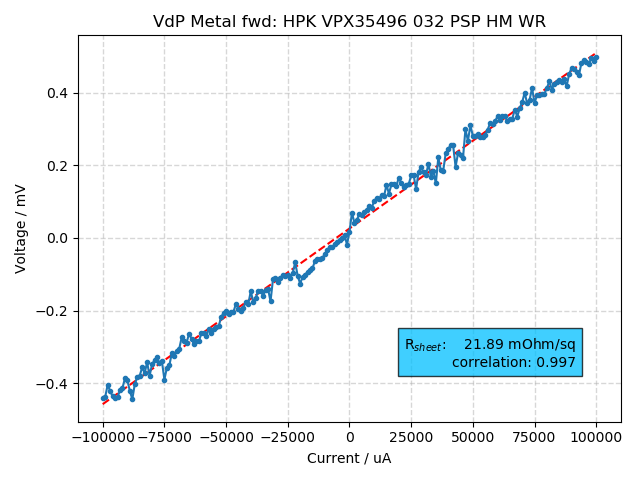
\includegraphics[width=6cm]{analysis/vdp_metal_fwd_HPK_VPX35496_032_PSP_HM_WR.png}
			};
			
			
			
		\end{tikzpicture}
	
	\end{frame}
	
	\begin{frame}
		\frametitle{\batch: Flute 4}
		




{# for some reason the relative path does not work, so we have to make do with the links #}

	\end{frame}


	
	\begin{frame}
		\frametitle{\batch: Summary}
		
		\begin{itemize}
			\item{ \color{dorange} Bulk resistivity low \color{dgreen}}
			\item{Breakdown structure: early breakdown, but DC process anyway}
			\item{\color{dgreen} p-stop/FET $V_{th}$ very homogeneous}
			
			\item{ \color{dgreen} Batch \batch \ can be accepted?}
		
		\end{itemize}
	\end{frame}
	
	
	
	
	
\end{document}